\chapter{Methodology}

\section{Pipeline}

\begin{figure}[H]
    \centering
    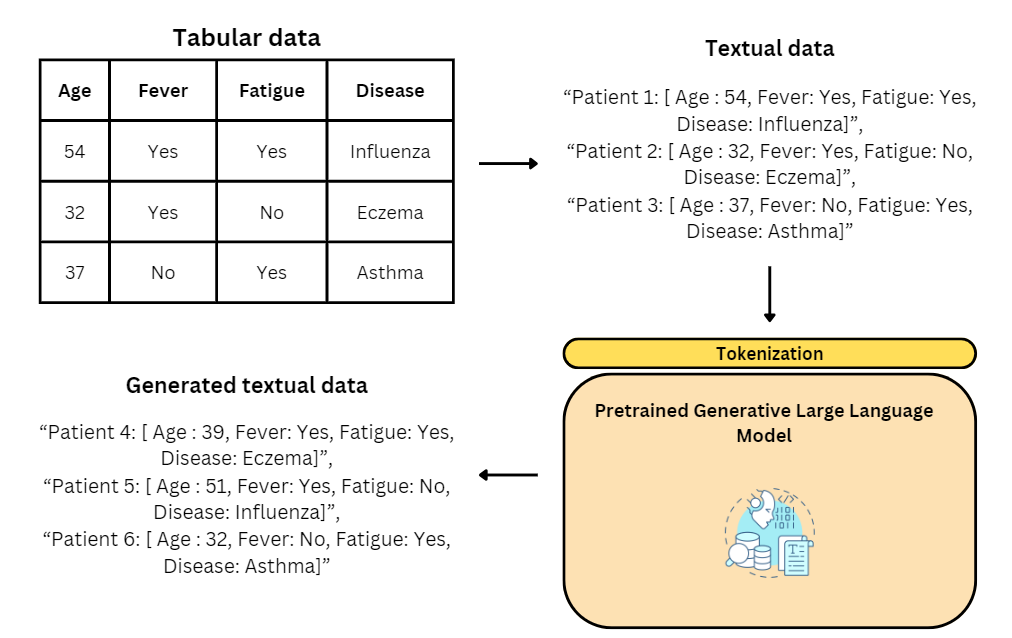
\includegraphics[width=0.85\textwidth]{images/pipeline.png}
    \caption{Data synthesis pipeline}
    \label{fig:pipeline}
\end{figure}

We propose a data synthesis pipeline consisting of several methodical steps. First, we propose to use two different datasets (small and large datasets) to evaluate the effectiveness of LLMs in generating data. This involves understanding how the data is going to be generated using LLMs. Then, a closer look is taken at the data to judge if it is essential to pre-process the data before using data synthesis methods. Next, state-of-the-art data generation models are leveraged to create high-fidelity synthetic data that closely resembles real-world information. Depending on the types of models utilized, they may give results in a different format than we initially wanted. In that case, post-processing is needed to convert the generated data into a CSV format. The CSV format will allow us to conduct a comparison and statistical analysis between the initial data and the generated one.

\section{Choices of Datasets}

In this paper, two datasets will be considered to ensure to validation of the results.
Given the ethical question around the manipulation of hospitals' data, the datasets used in this paper are publicly available and accessible via Kaggle.

\subsection{First Dataset}

The first dataset consists of 349 patients' health records in a CSV format (\cite{uom190346a_disease_symptoms_2021}). It contains 10 features including the patient's age, disease, and specific symptoms that are associated with the disease. 


This dataset quite is small given the number of patients. It will be used to generate the synthetic data, which is compared with the original data to perform statistical comparisons and also to train machine learning models to predict disease based on the other features.

It will be interesting to see how LLMs and GAN models can perform on such datasets.



\subsection{Second Dataset}

The second dataset consists of more than 4412 patients' health records (\cite{palivela_patient_treatment_2021}). It includes 11 features containing various haematological parameters measured in individuals, such as hematocrit, haemoglobin, erythrocyte count, leucocyte count, thrombocyte count, mean corpuscular haemoglobin (MCH), mean corpuscular haemoglobin concentration (MCHC), mean corpuscular volume (MCV), age, sex, and source of the sample (inpatient or outpatient). 

The second dataset is considered because the first dataset used is relatively small and might produce inaccurate generated results. Having a second dataset helps justify the results previously generated and it will be interesting to see how leveraging LLM power to provide relevant information based on such a large amount of information given initially.


\section{Choices of Models}

In our study, non-LLMs-based methods were utilized, more specifically, the model CTGAN (Conditional Tabular Generative Adversarial Network), inspired by Generative Adversarial Networks (GANs) adapted for data generation. The model is designed specifically for tabular data. Unlike other generative models that are often designed for image or text data, CTGAN is tailored to handle the unique challenges posed by tabular data, such as the presence of both continuous and categorical variables, and the need to maintain complex dependencies between columns (\cite{Xu2019}).


%A statistical model is used for data synthesis called Synthpop which is based on the R programming language.

%Both models mentioned above work directly with the CSV file being imported but with one particularity of being that Synthpop only works in R. 

%There is still a need, nonetheless, for pre-processing the data, more specifically, dealing with missing values, incoherent data formatting etc...

%%%%%%%%%%%%%%%%% CTGAN %%%%%%%%%%%%%%%%%%%%%%%%%%%%%%%%%%%%%%
\vspace{0.5cm}

\begin{figure}[ht!]
    \centering
    \begin{tikzpicture}[
        block/.style = {rectangle, draw, fill=blue!20, text width=6em, text centered, rounded corners, minimum height=5em},
        largerblock/.style = {rectangle, draw, fill=blue!20, text width=8em, text centered, rounded corners, minimum height=5em},
        line/.style = {draw, -latex, thick}, % Thicker lines and larger arrow tips
        textblock/.style = {text width=10em, text centered}
    ]
        % Nodes
        \node [block] (generator) {Generator};
        \node [largerblock, right=of generator, node distance=18cm] (discriminator) {Discriminator};
        \node [block, below=of generator, fill=green!20, node distance=8cm] (noise) {Noise};
        \node [largerblock, below=of discriminator, fill=red!20, node distance=8cm] (realdata) {Tabular Data};
        \node [largerblock, right=of discriminator, node distance=18cm] (output) {Synthetic Tabular Data};
        
        % Invisible nodes to extend arrows
        \node (gen_ext) [right=of generator, node distance=8cm] {};
        \node (disc_ext_left) [left=of discriminator, node distance=8cm] {};
        \node (disc_ext_right) [right=of discriminator, node distance=8cm] {};
        \node (out_ext) [left=of output, node distance=8cm] {};

        % Lines
        \path [line] (noise) -- (generator) node[midway, left] {Noise Input};
        \path [line] (generator.east) -- (gen_ext) -- (disc_ext_left) -- (discriminator.west) node[midway, above] {Fake Samples};
        \path [line] (realdata) -- (discriminator) node[midway, left] {Real Samples};
        \path [line] (discriminator.east) -- (disc_ext_right) -- (out_ext) -- (output.west) node[midway, above] {Evaluate};
    \end{tikzpicture}
    \caption{CTGAN Pipeline}
    \label{fig:gan_pipeline}
\end{figure}


CTGAN, just like GANs, is composed of two main components: a generator and a discriminator. They are trained simultaneously in a process where the generator tries to create synthetic data that is indistinguishable from real data, while the discriminator tries to distinguish between real and synthetic data.

\begin{itemize}
    \item[1.] \textsc{Generator}\\
    It takes random noise as input and generates synthetic data samples.

    \item[2.] \textsc{Discriminator}\\
    It evaluates the data samples and tries to classify them as real or synthetic. It provides feedback to the generator on how to improve the quality of the generated data.

    \item[3.] \textsc{Training} \\
    During training, the generator and discriminator are updated iteratively. The generator aims to minimize the probability of the discriminator correctly identifying the synthetic data, while the discriminator aims to maximize this probability. This adversarial training process continues until the discriminator can no longer distinguish between real and synthetic data effectively.
    
\end{itemize}


\vspace{1cm}

\noindent For the state-of-the-art LLMs, the following are the selected models:

\begin{itemize}
    \item[1.] \textsc{BeGreat model} \\
    The model is designed to generate synthetic data using LLMs. It specifically leverages the DistilGPT-2 model to fit and generate data. It is an open-source model, which makes it particularly suitable for creating anonymized data without compromising privacy (\cite{great_library_2024}).



    
    \item[2.] \textsc{LLaMa-3 model}, with 8 billion learning parameters.\\
    The open-source model, developed by Meta, is the state-of-the-art model for advanced text generation tasks. Available in two sizes 8 billion and 70 billion parameters, they are auto-regressive language models utilizing an optimized transformer architecture, which enhances their efficiency and scalability for various use cases (\cite{meta2024llama3, huggingface2024llama3}). Due to the computational limitations the model with 8 billion parameters.

    %\item Google's LLM called Gemma, 7 billion parameters version.
    %\item Mistral's LLM is called Mistral version 0.2 with 7 billion parameters.
\end{itemize}

\begin{figure}[H]
    \centering
    \begin{tikzpicture}[
        block/.style = {rectangle, draw, fill=blue!20, text width=5em, text centered, rounded corners, minimum height=3em},
        line/.style = {draw, -latex}, % Thicker lines and larger arrow tips
        node distance=1cm % Adjusted node distance for compactness
    ]
        % Nodes
        \node [block] (datainput) {Data Input};
        \node [block, right=of datainput] (embedding) {Embedding Layer};
        \node [block, right=of embedding] (encoder) {Encoder};
        \node [block, right=of encoder] (decoder) {Decoder};
        \node [block, right=of decoder] (output) {Output Layer};

        % Lines
        \draw [line] (datainput) -- (embedding);
        \draw [line] (embedding) -- (encoder);
        \draw [line] (encoder) -- (decoder);
        \draw [line] (decoder) -- (output);
    \end{tikzpicture}
    \caption{LLM Pipeline}
    \label{fig:llama3_pipeline}
\end{figure}

Such models require substantial computational resources; to address this, they are run on High-Performance Computation (HPC) clusters from the ADAPT Center. Nvidia's A100 GPUs 80GB within these clusters are utilized to run these state-of-the-art models efficiently.

Text-based prompts are the most prevalent approach for interacting with LLMs. More precisely, users provide a text prompt that explicitly describes what users want. They need to be clear enough so that LLMs can provide a high-quality and relevant response. Thus, more data pre-processing is necessary. As a matter of fact, the initial data is in tabular format which might infer with text prompts that the LLMs are receiving. We introduce thus, an additional data pre-processing that converts tabular data into textual data that we will go into detail later. 



\section{Data Pre-processing}

The data pre-processing encompasses a series of meticulous techniques aimed at transforming the initial dataset into a format that is interpretable by the data synthesis methods. This step plays a pivotal role as it ensures the quality and effectiveness of the data generation.

\vspace{0.5cm}
%%%%%%%%%%%%%%%%%%%%% INCONSISTENCIES %%%%%%%%%%%%%%%%%%%%%%%%

The initial data, when downloaded, might contain inconsistencies, errors, and missing values. The data cleaning process addresses these issues, which helps implement the data generative methods. In our cases, the process eliminates rows with missing information and fixes inconsistencies using the appropriate Python libraries.

\vspace{0.5cm}
%%%%%%%%%%%%%%%%%%% FURTHER LLMs %%%%%%%%%%%%%%%%%%%%%%%%%%%%%

Further data pre-processing is needed for the LLMs as the current data is in tabular format. A Python file class called TabularToTextualConverter is created, which includes a method called toTextual. It reads and converts each row and transforms it into a string containing all the features associated with that row. The associated features are separated by a comma which will help distinguish the different features for the LLMs. Thus, this method transforms tabular data into textual data. 

To illustrate the data pre-processing technique, consider the following dataset:

\begin{table}[H]
    \centering
    \renewcommand{\arraystretch}{1.5} % Increase cell height
    \setlength{\tabcolsep}{4pt} % Reduce column spacing
    \small % Reduce font size
    \begin{adjustbox}{max width=\textwidth}
    \begin{tabular}{|l|c|c|c|c|c|c|c|c|c|}
    \hline
    \makecell{\textbf{Disease}} & \makecell{\textbf{Fever}} & \makecell{\textbf{Cough}} & \makecell{\textbf{Fatigue}} & \makecell{\textbf{Difficulty} \\ \textbf{Breathing}} & \makecell{\textbf{Age}} & \makecell{\textbf{Gender}} & \makecell{\textbf{Blood} \\ \textbf{Pressure}} & \makecell{\textbf{Cholesterol} \\ \textbf{Level}} & \makecell{\textbf{Outcome} \\ \textbf{Variable}} \\ \hline
    Influenza & Yes & No & Yes & Yes & 19 & Female & Low & Normal & Positive \\ \hline
    \end{tabular}
    \end{adjustbox}
    \caption{Sample dataset with patient information}
    \label{table:sample_dataset}
\end{table}

After applying the data pre-processing steps described in our methodology, the transformed output for the first patient will be:

\begin{quote}
\textit{"Patient 1: [Disease: Influenza, Fever: Yes, Cough: No, Fatigue: Yes, Difficulty Breathing: Yes, Age: 19, Gender: Female, Blood Pressure: Low, Cholesterol Level: Normal, Outcome Variable: Positive]"}
\end{quote}

\vspace{0.5cm}

LLMs' input has a limit on the number of characters that they can accept. A method "getSubset" is created as a consequence, it subdivides the dataset into an equal number of subsets. 
Each request made for the LLM contains a subset of the dataset.

\begin{figure}[H]
    \centering
    \begin{tikzpicture}[
        block/.style = {rectangle, draw, fill=blue!20, text width=6em, text centered, rounded corners, minimum height=3em},
        smallblock/.style = {rectangle, draw, fill=blue!10, text width=4em, text centered, rounded corners, minimum height=2em},
        line/.style = {draw, -latex, thick}, % Thicker lines and larger arrow tips
        node distance=3cm % Adjusted node distance for compactness
    ]
        % Nodes
        \node [block] (dataset) {Dataset};
        \node [smallblock, below left=of dataset, xshift=-2cm] (subset1) {Subset 1};
        \node [smallblock, below=of dataset] (subset2) {Subset 2};
        \node [smallblock, below right=of dataset, xshift=2cm] (subsetn) {Subset n};

        % Dots for continuation
        \node[below right=of dataset, yshift=-0.5cm] (dots) {$\vdots$};
        
        % Lines
        \draw [line] (dataset) -- (subset1);
        \draw [line] (dataset) -- (subset2);
        \draw [line] (dataset) -- (subsetn);
    \end{tikzpicture}
    \caption{Dataset Subdivision}
    \label{fig:dataset_subdivision}
\end{figure}

More details of the implementation can be found in the following appendix \ref{app:tabTotext_appendix}.


%\section{High-Performance Computing (HPC) setup}

%The HPC, as its name suggests, is designed to deliver cutting-edge computational power for tackling complex tasks such as the LLMs. It is composed of a network of interconnected servers equipped with advanced processors, graphics cards and storage. However, when I came to utilise it, I did not go as planned. In fact, some code that runs flawlessly on my personal computer fails to execute on the HPC infrastructure. The reason why certain codes failed to perform on the HPC infrastructure is that they utilise an older version of Linux, coupled with outdated libraries that are incompatible with the code I am employing. I have to go through a long process of updating the libraries. If you are wondering, I did not code directly on the HPC terminal, but I have used instead a remote SSH with Microsoft Vscode. I wanted to write this section of this paper because it took a very long time to figure out the issues and try to fix them. 





\section{Data Post-processing}

\begin{figure}[H]
    \centering
    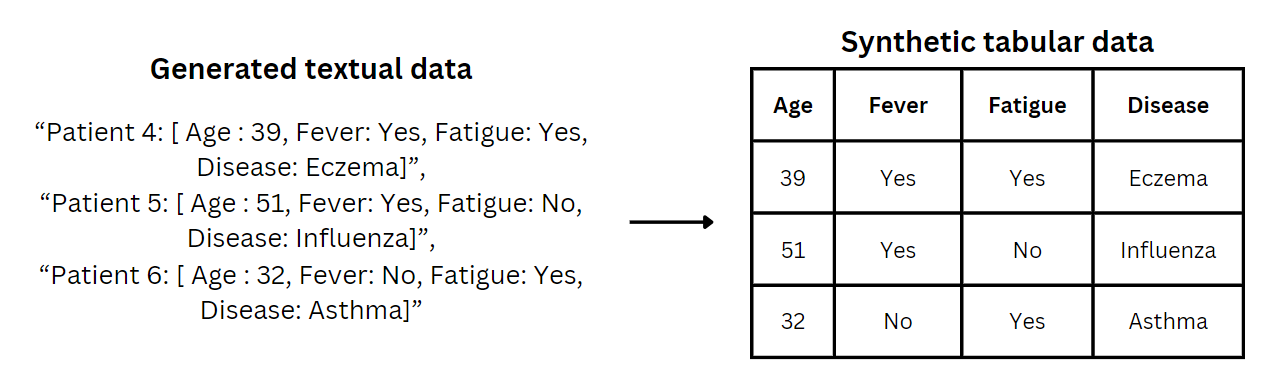
\includegraphics[width=0.85\textwidth]{images/textTotabular.png}
    \caption{Data synthesis pipeline}
    \label{fig:pipeline}
\end{figure}

The data post-processing deals with LLM responses which are stored in a TXT file. Unlike the data pre-processing, it also encompasses a series of meticulous techniques but, this time, it aims to transform the text file given by the LLMs into a CSV format file. The advantage of having a CSV file is to perform data analysis and compare it to the initial data. It will also help in comparing the models used and determining which is the one that performs the best. 

A Python class called TextualToTabularConverter is created, it is mainly based on regular expressions, to identify the matching patterns corresponding to the one that we specified in the text prompt given to the LLMs.
In cases where the regular expressions were not able to identify the patterns, because of the inconsistency of the LLMs' response, other pattern-matching methods are created specifically to identify the identify the exact pattern used by the LLMs.

More details of the implementation can be found in the following appendix \ref{app:textTotab_appendix}





% Define the specific LLM model and architecture to be used for data generation.

% Explain the data generation process, including data preparation, model training and evaluation

% Describe the metrics and evaluation criteria used to assess the quality adn realism of synthetic data.

% Discuss the potential biases and limitations of the chosen LLM model.






The evaluation of the results represents a critical part of the pipeline as it would determine if LLMs can provide performant results compared to GANs-based models.
However, it is important to select the right metrics to evaluate the data as they will be the ones that will judge if the data meets the quality standards and objectives of the analysis. The chosen metrics should align with the goals of the project and be capable of providing meaningful insights into the data's accuracy, relevance, and reliability.

\section{Evaluation}


As they are no official tools to measure how effective and safe is a synthetic data, there is, however, studies on how to empirically measure the effectiveness and the privacy. In this paper, we will be utilizing the state-of-the-art and complete Python framework called "Syntheval" to evaluate both the original and the synthetic data. %% ref to paper


\subsection{Measurement of the Similarity}

\begin{enumerate}
    \item Dimensionwise Means with 95\% of confidence intervals \\
    Scatter plots are utilized and the correlation confidence is measured to show how closely the synthetic data matches the values of the original data. 

    \item PCA Metrics \\
    The PCA eigenvalue difference is utilized to evaluate how well the synthetic data captures the variance and structure of the original data. A low value will indicate the model can capture the variance of the original data.

    \item Confidence Interval Overlap \\
    It measures how well the variability in the synthetic data matches the original data by comparing the overlap of their confidence intervals. A high value of the confidence interval overlap will show an inconsistency in preserving variability.

    \item Correlation Metrics \\
    The correlation matrix difference is calculated and it assesses how well the synthetic data preserves the relationships between variables in the original data. The smallest difference in correlation will show the best preservation of the relationships between the variables.

    \item Kolmogorov-Smirnov / Total Variation Distance Test \\
    The average combined statistics combine both Kolmogorov-Smirnov and Total Variation Distance Test values to evaluate the distributional similarity between synthetic and original data. A small average combined statistics will indicate the closest distributional match between the synthetic and original data.

    \item Empirical Hellinger Distance \\
    More precisely, the average Hellinger distance is calculated and it measures the similarity between probability distributions of the original and synthetic data. The smallest value of the average Hellinger distance will indicate the closest match to the original data’s distribution.

    \item Propensity Mean Squared Error (pMSE) \\
    pMSE evaluates how well the synthetic data mimics the original data for predictive modeling. A low value of the pMSE will show it effectively replicates the original data.

    \item Nearest Neighbour Adversarial Accuracy (NN Adversarial Accuracy)\\
    It assesses the distinguishability between synthetic and original data. A high value ensures the variability in distinguishability.

\end{enumerate}



\subsection{Measurement of the Accuracy of the Data}

In this section, the data and the synthetic data will be passed on to machine learning models to measure the accuracy. All models will be trained on the synthetic dataset and will be evaluated on the original dataset. The following machine learning models are utilized:

\begin{enumerate}
    \item Decision Tree Classifier \\
    A simple model, it can handle both numerical and categorical data.

    \item AdaBoost Classifier \\
    An improved version of the decision tree classifier focuses on the instances that are harder to classify and helps reduce the overall bias

    \item Random Forest Classifier \\
    The random forest classifier models are robust against overfitting as they leverage multiple decision trees.

    \item Logistic Regression \\
    Logistic regression is particularly effective for binary classification.
\end{enumerate}

\noindent Accuracy metrics are used to evaluate the generated data.

\begin{enumerate}
    \item Accuracy Real  (Acc R) \\
    It represents the classification accuracy of the original data. 

    \item Accuracy Fake (Acc F) \\
    It indicates the classification accuracy of the synthetic data.

    \item Absolute Difference ($|$Diff$|$) \\
    It shows the absolute difference between the accuracy real and the accuracy fake. This metric will show the discrepancy in the model's performance between the real and synthetic data.

    \item Error \\
    It represents the error rate of the model.
    
\end{enumerate}

\subsection{Measurement of the Data Privacy}


\begin{enumerate}
    \item Nearest Neighbour Distance Ratio \\
     It measures how close the synthetic data points are to the nearest real data points, with higher values indicating lower privacy.

    \item Median Distance to Closest Record \\
    measures the median distance from each synthetic data point to its nearest real data point, with higher values indicating better privacy.

    \item Hitting Rate (0.03 x Range(att)) \\
    It measures the fraction of synthetic data points that fall within a very small range of the real data points, with lower values indicating better privacy.

    \item Epsilon Identifiability Risk \\
    It measures the risk of re-identifying individuals in the synthetic data, with lower values indicating better privacy.

    \item Attribute Disclosure Risk (Accuracy) \\
    It measures the risk of accurately predicting sensitive attributes, with lower values indicating better privacy.
    
\end{enumerate}